% This is samplepaper.tex, a sample chapter demonstrating the
% LLNCS macro package for Springer Computer Science proceedings;
% Version 2.21 of 2022/01/12
%
\documentclass[runningheads]{llncs}
%
\usepackage[T1]{fontenc}
% T1 fonts will be used to generate the final print and online PDFs,
% so please use T1 fonts in your manuscript whenever possible.
% Other font encondings may result in incorrect characters.
%
\usepackage{graphicx}
% Used for displaying a sample figure. If possible, figure files should
% be included in EPS format.
%

% My packages
% ----
\usepackage{pgfplots}
\usepackage{color}
\usepackage{amsmath}
\usepackage{amssymb}
\usepackage{amsfonts}
\usepackage{comment}
\usepackage{tikz} % nice language for creating drawings and diagrams

\DeclareMathOperator{\sign}{sign}

\newtheorem{proposition}{Proposition}
\newtheorem{definit}{Definition}
\newtheorem{proof}{Proof}
% ----

% If you use the hyperref package, please uncomment the following two lines
% to display URLs in blue roman font according to Springer's eBook style:
%\usepackage{color}
%\renewcommand\UrlFont{\color{blue}\rmfamily}
%\urlstyle{rm}
%
\begin{document}
%
\title{
    % Relational Expressivity Coverage: Comparing Risk-Sensitive Criteria
    Relational Expressivity Coverage: Comparing Risk-Sensitive Criteria for SSP Problems
}
%
\titlerunning{Relational Expressivity Coverage: Comparing Risk-Sensitive Criteria}
% If the paper title is too long for the running head, you can set
% an abbreviated paper title here
%
% \author{First Author\inst{1}\orcidID{0000-1111-2222-3333} \and
% Second Author\inst{2,3}\orcidID{1111-2222-3333-4444} \and
% Third Author\inst{3}\orcidID{2222--3333-4444-5555}}
%
% \authorrunning{F. Author et al.}
% First names are abbreviated in the running head.
% If there are more than two authors, 'et al.' is used.
%
% \institute{Princeton University, Princeton NJ 08544, USA \and
% Springer Heidelberg, Tiergartenstr. 17, 69121 Heidelberg, Germany
% \email{lncs@springer.com}\\
% \url{http://www.springer.com/gp/computer-science/lncs} \and
% ABC Institute, Rupert-Karls-University Heidelberg, Heidelberg, Germany\\
% \email{\{abc,lncs\}@uni-heidelberg.de}}
%
\maketitle              % typeset the header of the contribution
%

\begin{abstract}
% Short Version
Markov Decision Processes (MDPs) are commonly used to model sequential decision-making under uncertainty. A notable subclass is the Stochastic Shortest Path (SSP) problem, in which an agent aims to reach a goal state, modeled as absorbing, while minimizing accumulated costs. Policies in SSPs induce the random variable accumulated cost and its corresponding probability distribution function, and decision criteria summarize these distributions into scalar values to guide policy comparison and define optimality.
In this work, we propose the \emph{Relational Expressivity Coverage} method, which quantifies a criterion's ability to represent preference relations through parameter variation. We apply this framework to the One-State Many-Actions (OSMA) problem and compare multiple risk-sensitive criteria from the literature in terms of their expressivity.

% Long Version
% Markov Decision Processes (MDPs) are widely used to model sequential decision-making problems where an agent interacts with an environment and outcomes are probabilistic. The Stochastic Shortest Path (SSP) is a special case of MDP in which the agent must drive the process to a goal state, modeled as an absorbing state, while minimizing costs.
% Solutions to an SSP, policies, induce the random variable accumulated cost and its corresponding probability distribution function; a decision criterion maps the random variable accumulated cost to a scalar value to enable policy comparison and define optimality. 
% Risk-averse criteria emphasize high costs, while risk-prone criteria emphasize low costs. Several risk-sensitive criteria have been proposed in the literature, including the Exponential Utility Function, Piecewise-linear Transformation, Mean-Variance, Value at Risk, and Conditional Value at Risk.
% Because different criteria evaluate policies in distinct ways, direct comparison is challenging and often relies on qualitative aspects such as algorithmic convergence, theoretical foundations, the structure of optimal policies, and parameter interpretability.
% In this work, we propose the \emph{Relational Expressivity Coverage} method to evaluate risk-sensitivity from the perspective of expressivity, that is, the ability of a criterion to represent the decision-maker’s preference relations. Our objective is to assess how extensively each criterion, through parameter adjustment, can replicate preference orderings over a set of policies. We apply this method to a simplified environment, the One-State Many-Actions (OSMA) problem, and compare several risk-sensitive criteria from the literature in terms of expressivity.

\keywords{Relational Expressivity Coverage \and Expressivity \and Stochastic Shortest Path \and Preferences \and Stochastic Dominance \and Exponential Utility Function \and Piecewise-linear Transformation \and Mean-Variance \and Value at Risk \and Conditional Value at Risk.}
\end{abstract}
%
% ---- Document ----
%

% ---- Introduction ----
\section{Introduction}\label{sec:intro}

Markov Decision Process (MDP) \cite{puterman2014markov} models sequential decision-making problems. Stochastic Shortest Path (SSP) \cite{bertsekas1991analysis} is a subclass of MDPs where the agent aims to reach an absorbing goal state while minimizing accumulated cost.

A policy assigns an action to each state, and an optimal policy minimizes the expected cumulative cost for risk-neutral decision-making, typically using dynamic programming \cite{puterman2014markov}. SSPs usually assume proper policies, those that reach the goal state with probability one.

Incorporating uncertainty is essential for modeling real-world scenarios, as risk sensitivity significantly influences decision-making. For instance, in autonomous vehicle navigation, accounting for uncertainties such as the unpredictable behavior of traffic participants and partially observed environments is crucial for ensuring safety and efficiency \cite{autonomous-pomdps2014}. Similarly, in autonomous exploration, in challenging environments such as caves and mines \cite{autonomous-exploration2025}.

To address risk-sensitive problems, there are several criteria in the literature, such as Exponential Utility Function \cite{howard1972risk,exp-utility-function}, Piecewise-linear Transformation method \cite{mihatsch2002risk,piecewise-linear}, Value at Risk (VaR) \cite{jorion2001value} and Conditional Value at Risk (CVaR) \cite{rockafellar2000optimization,artzner1999coherent,chow2015risksensitive}.

The discussion around the merits of various criteria is often limited to theoretical analysis, computational performance, or algorithmic improvements, lacking quantitative comparisons that provide decision makers with the intuition about which risk criterion best represents their preferences. To address this gap, we introduce the concept of expressivity, defined as the set of preferences induced by the policies of a given risk criterion. Expressivity is analyzed in three forms: full (matching all preference relations exactly), dominant (capturing only preferred decisions), and relational (preserving pairwise weak orderings). 

We propose the Relational Expressivity Coverage (REC) method to compare risk-sensitive criteria based on weak preference orderings over policy pairs. To demonstrate its use, we propose a simplified environment named One-State Many-Actions (OSMA) problem.

The paper is organized as follows: Section~\ref{sec:background} introduces key concepts of MDPs under risk-neutral and risk-averse settings. Section~\ref{sec:expressivity} presents expressivity concepts of full, dominant, and relational coverage. Section~\ref{sec:rel-expressivity-in-practice} presents the proposed metric for comparing risk criteria and applies the Relational Expressivity Coverage (REC) method to a simplified problem. Section~\ref{sec:results} reports the analytical and empirical results. Section~\ref{sec:conclusion} concludes and outlines future work.

% We propose the Relational Expressivity Coverage (REC) method to compare risk-sensitive criteria, constructing three regions: dominant, dominated, and configuration. While Configuration Regions quantify configurability, applying them across diverse problems is challenging; we demonstrate their applicability using the One-State Many-Actions (OSMA) problem.

\begin{comment}
The Markov Decision Process (MDP) \cite{puterman2014markov} models sequential decision-making problems. A Stochastic Shortest Path (SSP) \cite{bertsekas1991analysis} is a subtype of MDP where an agent selects actions in each time period with the objective of reaching an absorbing state, typically the goal state, while minimizing the accumulated cost. 

A policy associates, for each state, an action available for the agent to execute. Typically, an optimal policy selects actions that minimize the cumulative expected cost by employing dynamic programming techniques \cite{puterman2014markov}. It is common to consider SSP problems with proper policies, i.e., a policy that guarantees termination with probability one; it is also common to consider that every non-proper policy accumulates an infinite expected cost.

The incorporation of uncertainty into the environment is a critical aspect when modeling real-world problems, as the agent's decision-making is intricately linked to its sensitivity to risk. This sensitivity is particularly evident in real-life scenarios such as finance \cite{vittori2020option}. % Robotics and Autonomous Navigation.

To address risk-sensitive problems, there are several criteria in the literature, such as the Exponential Utility Function \cite{howard1972risk, exp-utility-function} that incorporates risk attitude by minimizing the expected exponential of accumulated costs. The Piecewise-linear Transformation method \cite{mihatsch2002risk, piecewise-linear} introduces a set of fixed-point operators with contraction properties, leveraging a Piecewise-linear Transformation function. Mean-Variance optimization \cite{markovitz-portfolio, sobelmeanvariance} is explored in dynamic optimization by identifying an optimal policy that balances the trade-off between minimizing the mean and variance of the costs. The Value at Risk (VaR) \cite{jorion2001value} estimates the maximum expected loss at a given confidence level, and the Conditional Value at Risk (CVaR) \cite{rockafellar2000optimization, artzner1999coherent, chow2015risksensitive} consider the average loss beyond the VaR threshold, addressing tail risk concerns; both measures have been adapted for MDPs, optimizing decision-making under uncertainty.

The discussion around the merits of various criteria is often isolated, lacking quantitative comparisons using formal methods. To address this, we introduce the concept of configurability, which measures how well a criterion captures the spectrum of a decision-maker’s preferences. Configurable criteria effectively represent the desired preferences by aligning with the decision-maker's risk sensitivity.

We propose the Configuration Regions (CR) method to compare risk-sensitive criteria, constructing three regions: dominant, dominated, and configuration. While Configuration Regions quantify configurability, applying them across diverse problems is challenging, we demonstrate their applicability using the One-State Many-Actions (OSMA) problem.

The remainder of this paper is structured as follows. Section 2, Background, introduces key definitions for Markov Decision Processes (MDPs) under both neutral and risk-averse conditions. Section 3, Expressivity and Configuration Region, presents the concepts related to preference modeling and discusses the proposed metric for comparing different risk criteria. Section 4, Configuration Region in the OSMA Problem, outlines the analytical approach of the Configuration Region (CR) method within a simplified problem. Section 5, Criteria Propositions for OSMA, details the propositions for each risk criterion under analysis. Section 6, Results, synthesizes the analytical and empirical findings related to the OSMA problem, focusing on the configurability of each risk criterion. Finally, Section 7, Conclusion, summarizes the paper's contributions and discusses directions for future research.
\end{comment}

% ----

% ---- Background ----
\section{Background} \label{sec:background}

The Stochastic Shortest Path (SSP) is a Markov Decision Process (MDP) defined by the tuple $\langle \mathcal{S}, \mathcal{A}, T, C, s_0, s_G \rangle$, where $\mathcal{S}$ and $\mathcal{A}$ are finite sets of states and actions, $T(s,a,s')$ gives the transition probability from $s$ to $s'$ under action $a$, and $C(s,a)$ defines the immediate cost of taking action $a$ in state $s$. The process starts in an initial state $s_0 \in \mathcal{S}$ and aims to reach a goal state $s_G \in \mathcal{S}$, which is absorbing $T(s_G,a,s_G) = 1$ and cost-free $C(s_G,a) = 0$. An SSP problem, together with a policy $\pi$, induces a Markov chain and a corresponding random variable $Z^\pi_s$, representing the accumulated cost from state $s$.

At each time step, the agent observes a state $s_t$, chooses an action $a_t$, transits to $s_{t+1}$ based on $T$, and incurs immediate cost $C(s_t, a_t)$. A policy $\pi: \mathcal{S} \rightarrow \mathcal{A}$ specifies the agent's action choice in each state.

\subsubsection{Risk-neutral Criterion}
The optimal policy, under the risk-neutral criterion, represented as $\pi^*$, can be obtained by minimizing the expected cumulative cost. The value function for a policy $\pi$ and a state $s$, denoted as $V^{\pi}(s)$, is defined as:
\begin{equation}
    V^\pi(s)= \lim_{T \to \infty} \mathbb{E} \left[\left.
    \sum_{t=0}^{T} C(s_{t}, a_{t}) \right| \pi, s_0 = s
    \right], \mbox{ for all } s \in \mathcal{S}.
\end{equation}

These concepts find application in risk-neutral planning, where the value function optimizes the expected overall cost of the policy. In contrast, in risk-averse planning, additional risk factors are introduced to capture the agent's risk attitude.

\subsubsection{Weak-order Preferences} We consider decision-makers that present a weak order on the set of policies $\Pi$, i.e., there exists a preference relation $\succeq$ (better or equal) that presents: transitivity ($a \succeq b \wedge b \succeq c \to a \succeq c$), reflexivity ($a \succeq a$), and totality ($a \succeq b \vee b \succeq a$). Note that any of the risk criteria here presented $\psi$ and risk factors $\omega$ produce a weak-order preference $\delta_{\psi,\omega}$.

\subsubsection{Stochastic Dominance} In decision theory, a lottery (i.e., a probability distribution over possible outcomes) is said to stochastically dominate another if it is universally preferred by a broad class of decision-makers under uncertainty. Let $F^\pi_s(z) = \Pr(Z^\pi_s \leq z)$ denote the cumulative distribution function (CDF) of the cost under policy $\pi$ from state $s$. Under First-Order Stochastic Dominance (FSD) \cite{hadar1969rules,bawa1975optimal}, policy $\pi$ is preferred to policy $\pi'$ in state $s$ (denoted $\pi \succeq \pi'$) if $F^\pi_s(z) \geq F^{\pi'}_s(z)$ for all $z \in \mathbb{R}$, with strict inequality for some $z$. In this case, policy $\pi$ is said to dominate policy $\pi'$ in state $s$.

\subsubsection{Certainty Equivalent} Consider a fictitious action $a_{G}$ that guides the process with probability 1 to the goal state and pays a constant cost $\widetilde{C}$. A constant cost $\widetilde{C}^{\pi}_{s}$ is the certainty equivalent of the random variable $Z^{\pi}_{s}$, if the decision-maker, when in state $s$, is indifferent between choosing $\pi$ or choosing action $a_{G}$ with $\widetilde{C} = \widetilde{C}^{\pi}_{s}$, i.e., regarding decision-maker preference, policy $\pi$ and action $a_{G}$ are equivalent and both options are considered equally preferable.

\subsubsection{Risk-Sensitivity} 
While dominance can be used to classify decision-makers regarding rationality, certainty equivalent can be used to classify decision-makers regarding risk sensitivity. A decision-maker is: 
\begin{itemize}
    \item \textbf{Risk-neutral} if $\widetilde{C}^{\pi}_{s} = V^{\pi}(s)$ for all policy $\pi$ and state $s$, i.e., there is no difference among policies that present the same expected accumulated cost;
    \item \textbf{Risk-averse} if $\widetilde{C}^{\pi}_{s} > V^{\pi}(s)$ for all policy $\pi$ and state $s$, i.e., the decision-maker accept paying a constant cost higher than some expected accumulated cost to avoid uncertainty; and
    \item \textbf{Risk-prone} if $\widetilde{C}^{\pi}_{s} < V^{\pi}(s)$ for all policy $\pi$ and state $s$, i.e., the decision-maker prefers experiencing the uncertainty, unless he pays a smaller cost than some expected accumulated cost. 
\end{itemize}

\subsubsection{Exponential Utility Method}
The Exponential Utility Method (EUM) \cite{howard1972risk,exp-utility-function} is based on Expected Utility Theory and assigns a scalar value to a policy by computing the expected exponential of the accumulated costs:
\begin{equation}
    V^\pi_{EUM}(s; \lambda) = \lim_{N \to \infty} \mathbb{E} \left[\left.
        \sign(\lambda) \exp\left(\lambda \sum_{t=0}^{N-1} C(s_t, a_t)\right) \right| \pi, s_0 = s
    \right].
\end{equation}
The risk sensitivity of the decision-maker is controlled by the parameter $\lambda$: positive values ($\lambda > 0$) indicate risk aversion, while negative values ($\lambda < 0$) indicate risk proneness. 

The magnitude of $\lambda$ reflects the intensity of the preference. However, if $\lambda$ exceeds a threshold denoted by $\lambda_{\text{extreme}}$, the expected cost may be infinite, and the method is not guaranteed to yield an optimal policy \cite{freire2016extreme}. Therefore, the method is valid for $\lambda \in [-\infty, \lambda_{\text{extreme}}]$. One way to compute $\lambda_{\text{extreme}}$ is to identify the largest value of $\lambda$ for which $V^\pi_{EUM}(s; \lambda)$ remains finite, ensuring the policy remains feasible.

\subsubsection{Piecewise-linear Transformation}
The Piecewise-linear Transformation (PLT) \cite{mihatsch2002risk,piecewise-linear} modifies the temporal difference update $x$, where $x = c_{t} + V(s_{t+1}) - V(s_{t})$, using a set of fixed-point operators with contraction properties. The transformation is defined by the function $\mathcal{X}^{(k)}(x)$, which adjusts the temporal difference as follows:
\begin{equation}
    \mathcal{X}^{(k)}(x) = 
    \left\{ \begin{array}{rcl}
    (1-k)x, & \mbox{if } x < 0, \mbox{ and} \\
    (1+k)x, & \mbox{otherwise.}
    \end{array}\right.,
\end{equation}
where $k \in [-1, 1]$ is the risk parameter. Positive values of $k$ correspond to risk aversion, while negative values represent risk proneness.

This transformation is applied within a modified Bellman equation to define the PLT value function:
\begin{equation}
        V^\pi_{PLT}(s; k) = \sum_{s' \in \mathcal{S}}
        T(s,\pi(s),s') \mathcal{X}^{(k)}
        (C(s,\pi(s)) + \alpha V_{PLT}^\pi(k, s') - V_{PLT}^\pi(k, s)).
\end{equation}

\subsubsection{Mean-Variance} The mean-variance (MV) \cite{sobelmeanvariance} is a relevant method in stochastic optimization, aiming to identify policies that balance expected performance with associated risk, involving optimizing a trade-off between the expected cumulative cost and the variability of that cost.

For a given policy $\pi$ and initial state $s$, the MV value function is defined as:
\begin{equation}
    V^{\pi}_{MV}(s; \mu) =  
    \mathbb{E} [ Z^{\pi}_{s} ] + \mu \sigma^2 [Z^{\pi}_{s}],
\end{equation}
where $Z^{\pi}_s$ is the total discounted cost from state $s$ under policy $\pi$; $\mu \geq 0$ reflects risk aversion, which penalizes variability; $\mu = 0$ is risk-neutral; and $\mu \leq 0$ reflects risk proneness.

\subsubsection{Value at Risk}
Value at Risk (VaR) \cite{jorion2001value} estimates the maximum expected loss at a given confidence interval. In the context of MDPs, define the VaR-based value function as:
\begin{equation}
    V^{\pi}_{VaR}(s; \alpha) = \mbox{min} \left\{
    z \mid Pr(Z^{\pi}_{s}) \geq (1 - \alpha)
    \right\},
\end{equation}
where $\alpha$ is defined by the range $\alpha \in [0, 1]$; $\alpha \geq 0.5$ indicates risk aversion; and $\alpha = 0.5$ indicates risk neutrality.

Here, $V^{\pi}_{VaR}(s; \alpha)$ represents the $\alpha$-quantile worst-case cost under policy $\pi$, meaning that with probability at least $1 - \alpha$, the cost will not exceed this value.

\subsubsection{Conditional Value at Risk}
Conditional Value at Risk (CVaR) quantifies the expected loss in the tail of the cost distribution beyond the VaR threshold, thus capturing exposure to rare but high-cost outcomes. Formally, it is defined as the expected value of $Z^{\pi}_s$ conditioned on the worst $\beta$-fraction of outcomes \cite{chow2015risksensitive}. The CVaR value function for a given confidence level $\beta \in (0, 1]$ is:

\begin{equation}
    V^{\pi}_{CVaR}(s; \beta) = \mathbb{E} \left[
    Z^{\pi}_{s} \mid Z^{\pi}_{s} \geq V^{\pi}_{VaR}(s; \beta)
    \right],
\end{equation}
where $Z^{\pi}_s$ is the cost random variable under policy $\pi$, and $V^{\pi}_{VaR}(s; \beta)$ is the corresponding Value at Risk.

The parameter $\beta$ controls the degree of risk sensitivity: values close to 1 represent strong risk aversion, while $\beta = 0.5$ corresponds to risk neutrality.

% ---- Background ----
\section{Expressivity Coverage: Full, Dominant and Relational}\label{sec:expressivity}

This section evaluates the expressive capacity of risk criteria in capturing a risk-sensitive decision-maker’s preferences within a stochastic decision process. The goal is to determine how well each criterion, through parameter adjustments, can reproduce the preference structure underlying policy orderings of an arbitrary decision-maker.

Formally, the expressiveness of a risk criterion $\psi \in \Psi$, with $\Psi$ equal to each risk criterion analyzed, is its ability to replicate the preference structure ordering over a policy set $\Pi$ for some parameter $\omega \in \Omega^\psi$, where $\Omega^\psi$ is the criterion’s parameter space.

The Full Expressivity Coverage (FEC) quantifies this ability, assuming complete knowledge of the decision-maker’s preferences. The set of all preference orderings reproducible by a given criterion is defined accordingly.

\begin{definition}
    Let $\psi$ be a risk criterion; ${\mathcal{M}}$ be a SSP problem; $\Omega^{\psi}$, the space of risk factors associated with $\psi$; $\Delta^{\psi}$, the set of weak order preferences that can be represented under the criterion $\psi$; $\delta$, a weak order preference in $\Delta^{\psi}$; and $V^{\omega}$, the value function parameterized by $\omega \in \Omega^{\psi}$, whose induced ordering over the set of policies is equivalent to the preference $\delta$. With these definitions, the Full Expressivity Coverage is formulated as:
    \begin{equation}
        \begin{aligned}
        \mathcal{F}^{\mathcal{M}}_\psi
        &= \bigl\{\delta\in\Delta^\psi \mid \exists\,\omega\in\Omega^\psi:\;V^\omega\equiv\delta\bigr\}.
        \end{aligned}
    \end{equation}
    where $V^\omega\equiv\delta$ denotes that the value function $V^\omega$ fully represents the preference structure captured by $\delta$.
    % The FEC assumes that $\mathcal{F}^{\mathcal{M}}_\psi = \Delta^\psi_{\mathcal{F}}$, as shown when:
    % \begin{equation}
    %     \begin{aligned}
    %     \mathcal{F}^{\mathcal{M}}_\psi = \Delta^\psi_{\mathcal{F}}
    %     \Longleftrightarrow \forall \delta \in \Delta^\psi, \exists \omega \in \Omega^\psi: V^\omega \equiv \delta.
    %     \end{aligned}
    % \end{equation}
\end{definition}

The comparison between criteria is based on the inclusion of sets: if $\mathcal{F}^{\mathcal{M}}_{\psi} \subseteq \mathcal{F}^{\mathcal{M}}_{\psi'}$, then $\psi'$ is at least as expressive as $\psi$.

\begin{definition}
    Let $\psi, \psi'$ be risk criteria, and let $\mathcal{F}^{\mathcal{M}}_{\psi}, \mathcal{F}^{\mathcal{M}}_{\psi'}$ denote the complete expressivity coverage of the criteria $\psi$ and $\psi'$, respectively. The preference relation between risk criteria is then established as
    \begin{equation}
        \psi \succeq \psi' \iff \mathcal{F}^{\mathcal{M}}_{\psi} \subseteq \mathcal{F}^{\mathcal{M}}_{\psi'}.
    \end{equation}
\end{definition}

Full Expressivity Coverage demands the risk criterion can accurately reflect the decision-maker's preference structure. However, this requirement can be relaxed through partial approaches. One such approach is Dominant Expressivity Coverage (DEC), which checks whether a policy $\pi$, among the set of policies $\Pi$, is optimal with respect to the other policies.

\begin{definition}
    Let $\psi$ be a risk criterion; ${\mathcal{M}}$ be a SSP problem; $\Omega^{\psi}$ the space of risk factors associated with $\psi$; $\Delta^{\psi}_{\mathcal{D}}$ the set of dominant weak order preferences; $\delta$ a weak order preference in $\Delta^{\psi}_{\mathcal{D}}$; $\Pi$ the set of admissible policies under this criterion; $\pi$ and $\pi'$ any policies in $\Pi$; and $V^{\omega}(\pi)$ the value function that evaluates policy $\pi$ according to the parameter $\omega \in \Omega^{\psi}$. With these definitions, dominant expressivity coverage is formulated as:
    \begin{equation}
        \begin{aligned}
        \mathcal{D}^{\mathcal{M}}_\psi
        &= \left\{ \pi \in \Pi
             \mid \exists \pi' \in \Pi , \exists\,\omega\in\Omega^\psi : V^{\omega}(\pi) \geq V^{\omega}(\pi')
        \right\}
        \end{aligned}
    \end{equation}
    % The Dominant Expressivity Coverage assumes that $\mathcal{D}^{\mathcal{M}}_\psi = \Delta^\psi_{\mathcal{D}}$, as shown when:
    % \begin{equation}
    %     \mathcal{D}^{\mathcal{M}}_\psi = \Delta^{\psi}_{\mathcal{D}}
    %     \quad\Longleftrightarrow\quad
    %     \forall\,\pi, \pi' \in \Pi,\;\exists\,\omega\in\Omega^\psi:\;V^{\omega}(\pi) \geq V^{\omega}(\pi').
    % \end{equation}
\end{definition}

\begin{definition}
    Let $\psi, \psi'$ be risk criteria, and let $\mathcal{D}_{\psi}, \mathcal{D}_{\psi'}$ denote the dominant expressivity coverage of criteria $\psi$ and $\psi'$, respectively. The preference relation between risk criteria is then established as
    \begin{equation}
        \psi \succeq \psi' \iff \mathcal{D}^{\mathcal{M}}_{\psi} \subseteq \mathcal{D}^{\mathcal{M}}_{\psi'}.
    \end{equation}
\end{definition}

However, the measurement of Full Expressivity Coverage is a challenging task, as it requires considering all weak order preference relations among all policies. Moreover, Dominant Expressivity Coverage introduces the difficulty of identifying optimal policies with respect to the entire set of policies.

To mitigate this complexity, the notion of Relational Expressivity Coverage is introduced. This approach limits the analysis to the ability of the risk criterion to express relative preferences between specific pairs of policies. Thus, it evaluates whether, for a given pair of policies $(\pi, \pi')$, there exist parameters of the risk criterion capable of representing, alternatively, both the dominance of $\pi$ over $\pi'$ and its inversion. This approach eliminates the need to reproduce complete ordering over the entire set of policies, focusing instead on the criterion's ability to represent preference judgments between specific pairs of policies.

\begin{definit}
    Let $\psi$ be a risk criterion; $\mathcal{M}$ be a SSP problem; $\Omega^{\psi}$, the space of risk factors associated with $\psi$; $\Pi$, the set of policies under this criterion; $\Gamma^{\psi} \subseteq \Pi \times \Pi$, the set of ordered pairs of policies for which the relational capability of the criterion is to be evaluated; $\pi$ and $\pi'$ any policies in $\Pi$; $\omega$ and $\omega'$ risk factors in $\Omega^{\psi}$; and $V_{\psi}^{\pi}(\omega)$ the value function that assigns a value to policy $\pi$ based on parameter $\omega$. With these definitions, the formulation of Relational Expressivity Coverage is given by:
    \begin{equation}
        \begin{aligned}
            \mathcal{R}^{\mathcal{M}}_\psi
            &= \bigl\{ 
                (\pi,\pi')\in \Gamma^{\psi} \;\big|\;
                \exists\, \omega, \omega' \in \Omega^{\psi}:
                \\
            &\hspace{3em}
                V^{\omega}(\pi) \geq V^{\omega}(\pi')
                \wedge
                V^{\omega'}(\pi) \leq V^{\omega'}(\pi')
            \bigr\},
        \end{aligned}
    \end{equation}
\end{definit}

\begin{definit}
    Let $\psi, \psi'$ be risk criteria and $\mathcal{R}^{\mathcal{M}}_{\psi}, \mathcal{R}^{\mathcal{M}}_{\psi'}$ the REC of $\psi$ and $\psi'$, respectively. The preference relation between the risk criteria is then given by
    \begin{equation}
        \psi \succeq \psi' \iff \mathcal{R}^{\mathcal{M}}_{\psi} \subseteq \mathcal{R}^{\mathcal{M}}_{\psi'}.
    \end{equation}
\end{definit}

In the following section, we propose the application of these definitions within a simplified scenario called One-State Many-Actions.

% ---- Configuration Region ----
\section{Relational Expressivity Coverage in Practice}\label{sec:rel-expressivity-in-practice}

We consider a simple SSP, the One-State Many-Actions (OSMA) problem. The OSMA problem has two states, i.e., $\mathcal{S} = \{s_0, s_G\}$. The agent chooses among multiple actions $\mathcal{A}$, where $\mathcal{A}$ is continuous; an action is fully specified by the pair $\langle p,c \rangle = \langle T(s_{0},a,s_{G}),C(s_{0},a)\rangle$ where $c \in [0, \infty]$ and $p \in [0, 1]$; note that $T(s_{0},a,s_{i})=1-p$. A policy corresponds to a single action $\pi = [\pi(s)] = [a_{\pi}]$, so that a policy can be represented by a pair probability-cost, i.e., $\pi = \langle p_{\pi},c_{\pi} \rangle$ and can be represented in a bi-dimensional space. 

The OSMA problem involves evaluating policies based on their probability of reaching a goal state. The CDF for a policy $\pi$ is denoted by $F^{\pi}_s(z)$. For the OSMA problem, this CDF can be expressed using the geometric progression of the probability of reaching the goal state:
\begin{equation}
    F^{\pi}_s(z) = \left( 1 - (1 - p)^{\left\lfloor {\frac{z}{c}} \right\rfloor} \right),
\end{equation}
where $p$ is the probability of reaching the goal state under policy $\pi$, $c$ is the cost for executing the policy $\pi$ and $z$ represents the number of steps to reach the goal.
% TIKZPICTURE - OSMA - CDF
\begin{figure}[ht]
    \centering
    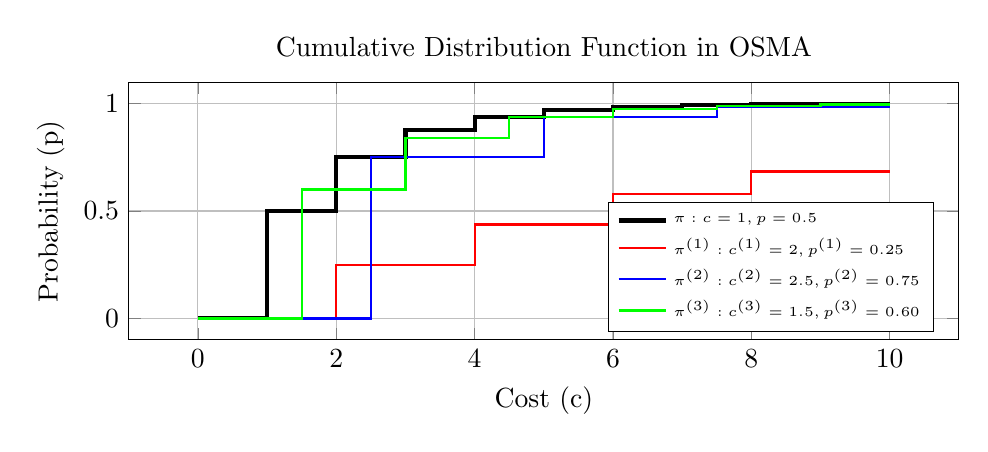
\begin{tikzpicture}
        \begin{axis}[
            width=\columnwidth, % Set the width to the text width
            height=0.4\columnwidth, % Adjust the height proportionally
            xlabel={Cost (c)},
            ylabel={Probability (p)},
            title={Cumulative Distribution Function in OSMA},
            legend pos=south east,
            legend style={font=\tiny, legend cell align=left}, % Reduce legend font size
            grid=major
        ]
        
        % \pi' curve (inverted)
        \addplot[line width=1.5pt, color=black, mark=none] coordinates {
            (0, 0) (1, 0) (1, 0.5) (2, 0.5) (2, 0.75) (3, 0.75) 
            (3, 0.875) (4, 0.875) (4, 0.9375) (5, 0.9375) 
            (5, 0.96875) (6, 0.96875) (6, 0.984375) (7, 0.984375)
            (7, 0.9921875) (8, 0.9921875) (8, 0.99609375) (9, 0.99609375)
            (9, 0.998046875) (10, 0.998046875) 
        };
        \addlegendentry{$\pi: c = 1, p = 0.5$};
        
        % \pi'' curve (inverted)
        \addplot[thick, color=red, mark=none] coordinates {
            (0, 0) (2, 0) (2, 0.25) (4, 0.25) (4, 0.4375) (6, 0.4375) 
            (6, 0.578125) (8, 0.578125) (8, 0.68359375) (10, 0.68359375)
        };
        \addlegendentry{$\pi^{(1)}: c^{(1)} = 2, p^{(1)} = 0.25$};
        
        % \pi'''' curve (inverted)
        \addplot[thick, color=blue, mark=none] coordinates {
            (0, 0) (2.5, 0) (2.5, 0.75) (5, 0.75) (5, 0.9375) (7.5, 0.9375)
            (7.5, 0.984375) (10, 0.984375)
        };
        \addlegendentry{$\pi^{(2)}: c^{(2)} = 2.5, p^{(2)} = 0.75$};
        
        % \pi''' curve (inverted)
        \addplot[thick, color=green, mark=none] coordinates {
            (0, 0) (1.5, 0) (1.5, 0.6) (3, 0.6) (3, 0.84) (4.5, 0.84)
            (4.5, 0.936) (6, 0.936) (6, 0.9744) (7.5, 0.9744)
            (7.5, 0.98976) (9, 0.98976) (9, 0.995904) (10, 0.995904)
        };
        \addlegendentry{$\pi^{(3)}: c^{(3)} = 1.5, p^{(3)} = 0.60$};
        
        \end{axis}
    \end{tikzpicture}
    \caption{Cumulative distribution function (CDF) in the OSMA problem for $\pi = \langle p=0.5, c=1 \rangle$, $\pi^{(1)} = \langle p^{(1)} = 0.25, c^{(1)} = 2 \rangle$, $\pi^{(2)} = \langle c^{(2)} = 2.5, p^{(2)} = 0.75 \rangle$ and $\pi^{(3)} = \langle p^{(3)} = 0.60, c^{(3)} = 1.5 \rangle$.}
    \label{fig:osma-cdf}
\end{figure}
% --------------------------------------------------------------------------------------

In Figure~\ref{fig:osma-cdf}, when comparing the weak order preference $\delta$ based on policy $\pi$, the following observations are made:
\begin{itemize}
    \item Policy $\pi$ exhibits first-order stochastic dominance (FSD) over $\pi^{(1)}$, since $p_{\pi} > p_{\pi^{(1)}}$ and $c_{\pi} < c_{\pi^{(1)}}$;
    \item Furthermore, $\pi$ also exhibits first-order stochastic dominance over $\pi^{(2)}$, as the CDF of $\pi$ is consistently greater than or equal to that of $\pi^{(2)}$, with specific values of $c$ where the CDFs of $\pi$ and $\pi^{(2)}$ coincide;
    \item Finally, the pair $\langle \pi, \pi^{(3)} \rangle$ belongs to $\mathcal{R}^{\mathcal{M}}_{\psi}$, since there is no dominance relationship between them.
\end{itemize}

When first-order stochastic dominance is not present, the Relational Expressivity Coverage is determined. Initially, the function $ f^{\pi}_{\psi}(p,c;\omega) := V^{\pi}_{\psi}(s; \omega) $ is defined for a given risk criterion $\psi$. The REC $\mathcal{R}^{\mathcal{M}}_{\psi}$ is then obtained through the curves $ f^{\pi}_{\psi}(p,c;\omega) = f^{\pi'}_{\psi}(p',c';\omega) $ across the entire space of risk parameters $\omega \in \Omega_{\psi}$.

Let $\omega^{+}_{\psi} = \sup (\Omega_{\psi})$ and $\omega^{-}_{\psi} = \inf (\Omega_{\psi})$. 
The Relational Expressivity Coverage $\mathcal{R}^{\mathcal{M}}_{\psi}$, illustrated in Figure~\ref{fig:regions-example}, 
is restricted between the following curves:
\begin{enumerate}
    \item $\lim_{\omega\to\omega^{+}_{\psi}} f^{\pi}_{\psi}(p,c;\omega) = \lim_{\omega\to\omega^{+}_{\psi}} f^{\pi'}_{\psi}(p',c';\omega)$, and
    \item $\lim_{\omega\to\omega^{-}_{\psi}} f^{\pi}_{\psi}(p,c;\omega) = \lim_{\omega\to\omega^{-}_{\psi}} f^{\pi'}_{\psi}(p',c';\omega)$.
\end{enumerate}
\begin{figure}[ht]
    \centering
    
\includegraphics[width=1\columnwidth]{img/equivalent_cost_full_area_colored.eps}
    \caption{Visual representation of the Relational Expressivity Coverage (REC), Dominated Expressivity Coverage (DEC), along with two synthetic asymptotic upper and lower bound functions.}
    \label{fig:regions-example}
\end{figure}

One approach to evaluate the Relational Expressivity Coverage $ \mathcal{R}^{\mathcal{M}}_{\psi} $ in the OSMA problem consists of analyzing the asymptotic behavior of the function $ f^{\pi, \pi'}_{\psi}(p, c; w) $ at the extremes defined by $ \omega^{+}_{\psi} $ and $ \omega^{-}_{\psi} $. This analysis allows constructing a bi-dimensional space of cost and probability, where the limiting curves drawn from these extremes delimit the region corresponding to the REC associated with the risk criterion $ \psi $.

Practically, in the next subsections, the propositions will be organized into four steps:
\begin{enumerate}
    \item \textbf{Value Function:} In this initial step, the value function associated with the risk criterion $ \psi $ is defined, applied to the specific problem $ \mathcal{M} = \text{OSMA} $. For a policy $ \pi $, characterized by a cost $ c $ and a success probability $ p $, the value function is represented as $ V^{\pi}_{\psi}(c,p;\omega) $, where $ \omega $ denotes the risk factor corresponding to the criterion $ \psi $. This function forms the basis for the other analyses by quantifying a policy's characteristics through the risk criterion.
    
    \item \textbf{Equivalent Cost:} The equivalent cost $ EC_{\psi}^{\pi} $ is determined such that the policy $ \pi $, with parameters $ (c, p) $, is considered equivalent, in terms of risk-adjusted value, to a hypothetical policy $ \pi' $, with parameters $ (c', p') $. This equivalence is expressed by the equality $ V^{\pi}_{\psi}(c,p;\omega) = V^{\pi'}_{\psi}(c',p';\omega) $. This step is essential for translating the perception of risk into comparable terms, allowing the identification of curves and expressivity coverage in the $ (p, c) $ space;
    
    \item \textbf{Asymptotic Lower Bound:} The limit function $ f_{\psi}^{\pi, \pi', -}(p,c;\omega^{-}) $ is defined, which describes the asymptotic behavior of the value function as the risk factor $ \omega $ approaches its lowest admissible value, i.e., when $ \omega \to \omega^{-}_{\psi} $. This function represents one of the boundaries of the REC of the criterion $ \psi $;
    
    \item \textbf{Asymptotic Upper Bound:} The limit function $ f_{\psi}^{\pi, \pi', +}(p,c;\omega^{+}) $ is defined, which describes the asymptotic behavior of the value function as the risk factor $ \omega $ approaches its highest admissible value, i.e., when $ \omega \to \omega^{+}_{\psi} $. This function represents one of the boundaries of the REC of the criterion $ \psi $;
\end{enumerate}

The following propositions, derived from each of the previously mentioned steps, will be presented in relation to the risk criteria of Exponential Utility Method (EUM), Piecewise-linear Transformation (PLT), Mean-Variance (MV), Value at Risk (VaR), and Conditional Value at Risk (CVaR).

%%%%%%%%%%%%%%%%%%%%%%%%%%%%%%%%%%%%%%%%%%%%%%%%%%%%%%%%%%%%%%%%%%%%%%%%
% Exponential Utility Function
%%%%%%%%%%%%%%%%%%%%%%%%%%%%%%%%%%%%%%%%%%%%%%%%%%%%%%%%%%%%%%%%%%%%%%%%
\subsection{Exponential Utility Method}

% PROPOSITIONS - EUM
\begin{proposition}
    Let $\psi = \text{EUM}$ be the risk criterion related to the Exponential Utility Method; $\omega = \lambda$ the risk factor associated with the risk criterion $\psi$; $\pi$ the policy; $c$ the cost paid to execute an action $a$ of the policy $\pi$; and $p$ the probability of success for transitioning to the target state.
    \begin{enumerate}
        \item \textbf{Value Function:} The value function quantifies the expected utility adjusted for risk for the policy $\pi$. In the case of the Exponential Utility Method, this function takes the form:
        \begin{equation}
            V^{\pi}_{EUM}(c, p; \lambda) = \frac 
            {\sign(\lambda) e^{\lambda c} p}
            {(1 - e^{\lambda c}(1 - p))}
        \end{equation}

        \item \textbf{Equivalent Cost:} This step determines the equivalent cost $EC^{\pi}_{EUM}$ that an alternative policy $\pi'$ must have to be considered equivalent to policy $\pi$, in terms of risk-adjusted value. The equivalence is guaranteed by the equality of the policy values under the EUM criterion:
        \begin{equation}
            EC^{\pi, \pi'}_{EUM}(c, p, p'; \lambda) = \log \left[ 
            \frac
                {e^{\lambda c} p}
                {p' - e^{\lambda c} p' + e^{\lambda c}p}
            \right] 
            \frac{1}{\lambda}.
        \end{equation}

        \item \textbf{Asymptotic Lower Bound:} When considering the limit $\lambda \to -\infty$, a behavior highly prone to risk is modeled, where only the best possible outcome is valued. In this case, the equivalent cost tends to the cost of the reference policy:
        \begin{equation}
            f^{\pi, \pi', -}_{EUM}(EC^{\pi, \pi'}_{EUM}; \lambda) = c.
        \end{equation}

        \item \textbf{Asymptotic Upper Bound:} In the limit $\lambda \to \lambda_e$, an extremely risk-averse behavior is assumed, where the worst outcomes are considered with maximum weight. The resulting limit function relates the costs and probabilities of the two policies logarithmically:
        \begin{equation}
            f^{\pi, \pi', +}_{EUM}(EC^{\pi, \pi'}_{EUM}; \lambda) = \frac{c \log(1-p')}{\log(1-p)}.
        \end{equation}
    \end{enumerate}
\label{prop:osma-eum}
\end{proposition}

%%%%%%%%%%%%%%%%%%%%%%%%%%%%%%%%%%%%%%%%%%%%%%%%%%%%%%%%%%%%%%%%%%%%%%%%
% Piecewise-linear Transformation
%%%%%%%%%%%%%%%%%%%%%%%%%%%%%%%%%%%%%%%%%%%%%%%%%%%%%%%%%%%%%%%%%%%%%%%%

\subsection{Piecewise-linear Transformation}

\begin{proposition}\label{prop:osma-plt}
    Let $\psi = \text{PLT}$ be the risk criterion related to the \textit{Piecewise-Linear Transformation}; $\omega = k$ the risk factor. The detailed definitions for each component and function are analogous to those found in Proposition~\ref{prop:osma-eum}.
    \begin{enumerate}
        \item \textbf{Value Function:}
        \begin{equation}
            V^{\pi}_{PLT}(c, p; k) = \frac{c (k - 2kp + 1)}{p (1 - k)}.
        \end{equation}
        
        \item \textbf{Equivalent Cost:}
        \begin{equation}
        EC^{\pi, \pi'}_{PLT}(c, p, p'; k) =  \frac
                    {c p' (k (1 - 2 p) + 1)}
                    {p (k (1 - 2 p') + 1)}.
        \end{equation}
        
        \item \textbf{Lower Asymptotic Function:} When considering the limit $k \to -1$, a behavior extremely prone to risk is modeled.
        \begin{equation}
            f^{\pi, \pi', -}_{PLT}(EC^{\pi, \pi'}_{PLT}; k) = c.
        \end{equation}
        
        \item \textbf{Upper Asymptotic Function:} In the limit $k \to +1$, an extremely risk-averse behavior is assumed.
        \begin{equation}
            f^{\pi, \pi', +}_{PLT}(EC^{\pi, \pi'}_{PLT}; k) = 
            \frac
            {c p' (1 - p)}
            {p (1 - p')}.
        \end{equation}
    \end{enumerate}
\end{proposition}

%%%%%%%%%%%%%%%%%%%%%%%%%%%%%%%%%%%%%%%%%%%%%%%%%%%%%%%%%%%%%%%%%%%%%%%%
% Mean-variance (MV)
%%%%%%%%%%%%%%%%%%%%%%%%%%%%%%%%%%%%%%%%%%%%%%%%%%%%%%%%%%%%%%%%%%%%%%%%

\subsection{Mean-variance (MV)}

\begin{proposition}\label{prop:osma-mv}
    Let $\psi = \text{MV}$ be the risk criterion related to the Mean-Variance; $\omega = \mu$ the risk factor. The detailed definitions for each component and function are analogous to those found in Proposition~\ref{prop:osma-eum}.
    \begin{enumerate}
        \item \textbf{Value Function:}
        \begin{equation}
            V^{\pi}_{MV}(c, p; \mu) = \frac{c}{p} + \frac{\mu c^2 (1 - p)}{p^2}.
        \end{equation}
        
        \item \textbf{Equivalent Cost:}
        \begin{equation}
            \begin{aligned}
                EC^{\pi, \pi'}_{MV}(c, p, p'; \mu) =\ 
                & \frac{-p'}{2 \mu (1 - p')} \nonumber \\
                & + \frac{p' \sqrt{1 + \frac{4 \beta (1 - p')}{p^2 p'^2} \cdot \left(p c + \mu (c)^2 (1 - p)\right) \cdot (p')^2}}{2 \mu (1 - p')}.
            \end{aligned}
        \end{equation}
        
        \item \textbf{Lower Asymptotic Function:} When considering the limit $\mu \to -p/c$, a behavior extremely prone to risk is modeled.
        \begin{equation}
            f^{\pi, \pi', -}_{MV}(EC^{\pi, \pi'}_{MV}; \mu) = c.
        \end{equation}
        
        \item \textbf{Upper Asymptotic Function:} In the limit $\mu \to \infty$, an extremely risk-averse behavior is assumed.
        \begin{equation}
            f^{\pi, \pi', +}_{MV}(EC^{\pi, \pi'}_{MV}; \mu) = 
            \frac{c p' \sqrt{1 - p}}{p \sqrt{1 - p'}}.
        \end{equation}
    \end{enumerate}
\end{proposition} 

\subsection{Value at Risk (VaR)}

\begin{proposition}\label{prop:osma-var}
    Let $\psi = \text{VaR}$ be the risk criterion related to the Value at Risk; $\omega = \alpha$ the risk factor. The detailed definitions for each component and function are analogous to those found in Proposition~\ref{prop:osma-eum}.
    \begin{enumerate}
        \item \textbf{Value Function:}
        \begin{equation}
            V^{\pi}_{VaR}(c, p; \alpha) = c  
            \left\lceil \frac{\log{\alpha}}{\log{(1-p)}} \right\rceil.
        \end{equation}
        
        \item \textbf{Equivalent Cost:}
        \begin{equation}
                EC^{\pi, \pi'}_{VaR}(c, p, p'; \alpha) = c \frac
                    { \left\lceil \frac{\log(\alpha)}{\log(1 - p)} \right\rceil }
                    { \left\lceil \frac{\log(\alpha)}{\log(1 - p')} \right\rceil }.
        \end{equation}
        
        \item \textbf{Lower Asymptotic Function:} When considering the limit $\alpha \to 0$, a behavior extremely prone to risk is modeled.
        \begin{equation}
            f^{\pi, \pi', -}_{VaR}(EC^{\pi, \pi'}_{VaR}; \alpha) = c.
        \end{equation}
        
        \item \textbf{Upper Asymptotic Function:} In the limit $\alpha \to 1$, an extremely risk-averse behavior is assumed.
        \begin{equation}
            f^{\pi, \pi', +}_{VaR}(EC^{\pi, \pi'}_{VaR}; \alpha) = 
            \frac
            {c \log{(1-p')}}
            {\log{(1-p)}}.
        \end{equation}
    \end{enumerate}
\end{proposition} 

%%%%%%%%%%%%%%%%%%%%%%%%%%%%%%%%%%%%%%%%%%%%%%%%%%%%%%%%%%%%%%%%%%%%%%%%
% Conditional at Risk (VaR)
%%%%%%%%%%%%%%%%%%%%%%%%%%%%%%%%%%%%%%%%%%%%%%%%%%%%%%%%%%%%%%%%%%%%%%%%

\subsection{Conditional Value at Risk (CVaR)}

\begin{proposition}\label{prop:osma-cvar}
    Let $\psi = \text{CVaR}$ be the risk criterion related to the Conditional Value at Risk; $\omega = \beta$ the risk factor. The detailed definitions for each component and function are analogous to those found in Proposition~\ref{prop:osma-eum}.
    \begin{enumerate}
        \item \textbf{Value Function:}
        \begin{equation}
            V^{\pi}_{CVaR}(c, p; \beta) = c \left( N + \frac{(1 - p)^{N}}{p} \right),
        \end{equation}
        where $N$ is calculated as the sum of $n$ terms in a geometric progression, with $n$ corresponding to the number of steps required for the accumulated probability of reaching the goal state to exceed the specified threshold.
        
        \item \textbf{Equivalent Cost:}
        \begin{equation}
                EC^{\pi, \pi'}_{CVaR}(c, p, p'; \beta) = 
                \frac{c p'}{p} \cdot
                    \left( 
                        \frac
                        {N p + (1 - p)^{N}}
                        {N' p' + (1 - p')^{N'}}
                    \right).
        \end{equation}
        
        \item \textbf{Lower Asymptotic Function:} When considering the limit $\beta \to 0$, a behavior extremely prone to risk is modeled.
        \begin{equation}
            f^{\pi, \pi', -}_{CVaR}(EC^{\pi, \pi'}_{CVaR}; \beta) = c.
        \end{equation}
        
        \item \textbf{Upper Asymptotic Function:} In the limit $\beta \to 1$, an extremely risk-averse behavior is assumed.
        \begin{equation}
            f^{\pi, \pi', +}_{CVaR}(EC^{\pi, \pi'}_{CVaR}; \alpha) = 
            \frac
            {c \log( 1 - p')}
            { \log(1 - p) }.
        \end{equation}
    \end{enumerate}
\end{proposition} 

% ---- Results ----
\section{Results}\label{sec:results}

% In this section, we assess the capacity of the asymptotic lower and upper bound functions, $f_{\psi}^{-}(p,c)$ and $f_{\psi}^{+}(p,c)$, to characterize relational expressivity coverage for five distinct risk criteria. We then undertake a comparative analysis to identify which criterion affords the greatest expressivity. Furthermore, we investigate the correspondence between the PLT method’s relational expressivity coverage and its cumulative distribution function (CDF) results, demonstrating that PLT yields policy recommendations that contravene the theoretical requirements of stochastic dominance.

This section evaluates the ability of the asymptotic bounds $f^{\pi, \pi', -}_{\psi}$ and $f^{\pi, \pi', +}_{\psi}$ to characterize relational expressivity for five risk criteria. We compare their expressivity and examine how the PLT method's results align with its CDF, showing that it can violate stochastic dominance principles.

\subsection{Comparative Analysis of Risk Criteria Based on Relational Expressivity Coverage}
\label{subsec:comparison_expressivity}

We first evaluate and compare the relational expressivity coverage achieved by each risk criterion. To this end, we use the propositions defined in Section~\ref{sec:rel-expressivity-in-practice} to construct the REC set $\mathcal{R}^{\mathcal{M}}_\psi$. These methods offer a quantitative approach to assess how well a risk criterion can represent the preferences of decision makers by varying the risk factor parameter.

In this context, given two risk criteria, $\psi$ and $\psi'$, a comparative assessment of their REC can be performed by evaluating the quantity $\mathcal{W}_{\psi}$. Specifically, $\psi$ is considered more expressive than $\psi'$ if $\mathcal{W}_{\psi} > \mathcal{W}_{\psi'}$, where
\begin{equation}
    \mathcal{W}^{\mathcal{M}}_{\psi} = \int_{p_{\mathrm{MIN}}}^{p_{\mathrm{MAX}}} \left| f^{\pi, \pi', -}_{\psi} - f^{\pi, \pi', +}_{\psi} \right| dp.
\end{equation}
Given that the OSMA problem involves only two decision variables, probability $p$ and cost $c$, the integral is computed with respect to the probability $p$ for a fixed value of $c$, thereby capturing the range of preference reversibility across the probability dimension.

To enable computation across all risk criteria $\psi$, we fixed the integration bounds at $p_{\mathrm{MIN}} = 0.01$ and $p_{\mathrm{MAX}} = 0.99$. Under this setup, the REC of each criterion, measured by the integral of the difference between its asymptotic bound functions, yields the following expressivity ordering:
\begin{equation}
    \mathcal{W}^{\mathcal{M}}_{\text{PLT}} > \mathcal{W}^{\mathcal{M}}_{\text{MV}} > \mathcal{W}^{\mathcal{M}}_{\text{EUM}} = \mathcal{W}^{\mathcal{M}}_{\text{VaR}} = \mathcal{W}^{\mathcal{M}}_{\text{CVaR}}.
\end{equation}
Accordingly, the corresponding REC rankings are given by:
\begin{equation}
    \mathcal{R}^{\mathcal{M}}_{\text{PLT}} \succ \mathcal{R}^{\mathcal{M}}_{\text{MV}} \succ \mathcal{R}^{\mathcal{M}}_{\text{EUM}} \equiv \mathcal{R}^{\mathcal{M}}_{\text{VaR}} \equiv \mathcal{R}^{\mathcal{M}}_{\text{CVaR}}.
\end{equation}

Another approach to comparing risk criteria in terms of \emph{Relational Expressivity Coverage} is to assess whether the upper and lower bound functions of one criterion are entirely contained within those of another. Specifically, a criterion $\psi$ is considered more expressive or equally expressive than $\psi'$ if, for all $p \in [p_{\text{MIN}}, p_{\text{MAX}}]$, the lower bound function of $\psi$ satisfies $f^{\pi, \pi', -}_{\psi} \geq f^{\pi, \pi', -}_{\psi'}$ when $p > p'$, and $f^{\pi, \pi', -}_{\psi} \leq f^{\pi, \pi', -}_{\psi'}$ when $p < p'$. Similarly, the same conditions must hold for the upper bound functions, such that $f^{\pi, \pi', +}_{\psi} \leq f^{\pi, \pi', +}_{\psi'}$ when $p > p'$, and $f^{\pi, \pi', +}_{\psi} \geq f^{\pi, \pi', +}_{\psi'}$ when $p < p'$.

As demonstrated by both approaches, and visually illustrated in Figure~\ref{fig:rec-by-risk-criterion}, the results indicate that the risk criterion $\psi = \text{PLT}$, with the risk factor $\omega = k$ from the Piecewise-Linear Transformation method, exhibits the highest relational expressivity for the OSMA problem.
\begin{figure*}[t]
    \centering
    
\includegraphics[width=1\textwidth]{img/English_relational_expressivity_coverage.eps}%{img/English_regiao_configuracao_por_metodo.png}
    \caption{Relational expressivity coverage results for the five analyzed risk criteria.}
    \label{fig:rec-by-risk-criterion}
\end{figure*}

\subsection{Piecewise-linear Transformation and Stochastic Dominance}
\label{subsec:plt_and_fsd}

In the previous subsection, we observed that the PLT method exhibits the highest Relational Expressivity Coverage. However, as discussed in Section~\ref{sec:background}, policies that are first-order stochastically dominated (FSD) cannot be preferred by a rational decision-maker, as they are suboptimal under any monotonic preference structure.

By comparing the cumulative distribution functions (CDFs) in the OSMA problem with the resulting REC produced by the PLT method, we found that PLT does not adhere to the principles of FSD, as shown in Figure~\ref{fig:plt-vs-cdf}. Specifically, it includes in its coverage set policies that are stochastically dominated, which violates fundamental rationality assumptions in decision theory.
\begin{figure}[t]
    \centering
    
\includegraphics[width=1\columnwidth]{img/English_regiao_configuracao_maior_igual_0.5.eps}
    \caption{Relational Expressivity Coverage for PLT and EUM are compared against the CDF curve.} % The plot reveals that the PLT coverage area lies above the CDF curve, indicating a violation of rationality assumptions commonly upheld in decision theory.
    \label{fig:plt-vs-cdf}
\end{figure}

%%%%%%%%%%%%%%%%%%%%%%%%%%%%%%%%%%%%%%%%%%%%%%%%%%%%%%%%%%%%%%%%%%%%%%%%
% Conclusion
%%%%%%%%%%%%%%%%%%%%%%%%%%%%%%%%%%%%%%%%%%%%%%%%%%%%%%%%%%%%%%%%%%%%%%%%

% ---- Conclusion ----
\section{Conclusion}\label{sec:conclusion}

In this work, the primary focus is on formally defining the Relational Expressivity Coverage (REC) method, specifically tailored for assessing the expressivity of different risk criteria. To thoroughly evaluate this method, we apply it within the context of the One-State Many-Action (OSMA) problem, proposing formal value functions for the four criteria under analysis.

The results highlight the Piecewise-linear Transformation method, particularly when employing the $k$ criterion, as the most configurable for addressing the risk-sensitivity inherent in the OSMA problem. By leveraging the REC method, we strive to offer a rigorous and quantitative comparison.

Additionally, when comparing the PLT method with the CDF of the analyzed policy, a critical aspect of PLT emerges. The method can generate policies that are first-order stochastically dominated by the reference policy, thereby not aligning with the rational preferences of the decision-maker.

While our analysis effectively evaluates the configurability of risk criteria within the OSMA context, this application is limited by its simplicity, featuring few states and straightforward decision-making. Future research could explore more complex environments and diverse risk criteria to ensure the robustness and validity of our conclusions.

% ---- Bibliography ----
%
% BibTeX users should specify bibliography style 'splncs04'.
% References will then be sorted and formatted in the correct style.
%
\bibliographystyle{splncs04}
\bibliography{ref}

\end{document}
